%% The CSAIL abstract book is a custom document class called 
%% "csailabstractbook".  It is based on the teTeX 1.0 distribution of LaTeX,
%% insofar as it uses a number of additional packages from teTeX for its
%% behind-the-scenes formatting. If you are using a different
%% distribution of LaTeX, it is possible that your distribution does not
%% have the necessary packages, in which case you will receive a missing 
%% package error when using the class file. You may wish to latex a copy 
%% of this file as-is to ensure that your configuration is correct.  

%% You should *not* include additional packages in preparing your
%% abstract.  The csailabstractbook class automatically includes the
%% standard "graphicx" package for inclusion of figures. An example of
%% its syntax is given in the text below, and more detailed documentation
%% can be found from the lab's latex page. Please use PDF files for your images.

%% Producing your abstract should be straightforward. Keeping all your
%% files in your working directory, run latex on the abstract file, bibtex
%% on the abstract file, and then latex on the abstract file twice.

\documentclass{csailabstractbook}
\usepackage{mathptm}

\begin{document}

%% The use of the sectioning commands, \abstitle and \absection, should 
%% be clear.  Try to follow the form of the sample text below, except
%% that your text should make a bit more sense.  It is ok to delete a 
%% section if it doesn't apply to your work.


\abstitle{Domain-Specific Optimization of Stream Programs}
         {Andrew Lamb, William Thies, and Saman Amarasinghe}

%% Please include an index entry for each author, keeping the names
%% consistent across abstracts. 
\index{Lamb, Andrew}
\index{Thies, William}
\index{Amarasinghe, Saman}

\absection{What}

We are building a suite of domain-specific optimizations that
incorporates the knowledge of expert DSP programmers to improve the
performance of high-level stream programs.  This work is in the
context of StreamIt~\cite{streamit-www}, an architecture-independent
programming language for high-performance streaming applications.  A
program in StreamIt is comprised of a set of concurrently executing
filters, each of which contains its own address space and communicates
with its neighbors using FIFO queues.  StreamIt aims to improve
programmer productivity by providing natural abstractions for stream
programming, as well as aggressive compiler optimizations that
eliminate the performance penalty that is typically associated with a
high-level programming model.
	
Our recent work has focused on optimizing portions of the stream
graph which are ``linear''~\cite{lamb-thesis,lamb03}.  A linear filter
is one in which every output is a linear combination of the inputs.
Linear components are common in DSP applications; examples include FIR
filters, expanders, compressors, FFTs and DCTs.  We have developed a
dataflow analysis that automatically recognizes linear filters.  Using
an abstract representation of linear filters, we show how to perform
algebraic simplification of adjacent linear nodes, as well as
automatic translation into the frequency domain.  These algorithmic
transformations, traditionally hand-tuned by DSP experts, are
completely automated in the StreamIt compiler and lead to a 450\%
performance improvement over our benchmark suite.

\absection{Why} 

Everything from cell phones to HDTV systems to satellite radios
require increasingly sophisticated algorithms for digital signal
processing. Optimization is especially important in this domain, as
embedded devices commonly have high performance requirements and tight
resource constraints.  Consequently, the current development process
that is embraced in industry has two stages: first, the algorithm is
designed and simulated at a high level of abstraction, and second, it
is optimized and reimplemented at a low level by an expert DSP
programmer.  In order to achieve high performance, the DSP programmer
needs to take advantage of global properties of the application that
could be exploited to obtain algorithmic speedups. Apart from
requiring expert knowledge, this effort is time-consuming,
error-prone, and costly, and must be repeated for every adjustment to
the high-level system design.  As embedded applications continue to
grow in complexity, these factors will become unmanageable.

One of the most common optimization targets of DSP experts are linear
sections of the stream graph.  In particular, neighboring linear nodes
can be combined into one, and large linear nodes can benefit from
translation into the frequency domain.  However, these optimizations
require detailed mathematical analysis and are tedious and complex to
implement.  They are only beneficial under certain
conditions---conditions that might change with the next version of the
system, or that might depend on neighboring components that are being
written by other developers.  To improve the modularity, portability,
and extensibility of stream programs, the compiler should be
responsible for identifying linear nodes and performing the
appropriate optimizations.

\absection{How}

The linear optimizations in StreamIt operate an abstract
representation of linear nodes (see Figure~\ref{fig:thies3-node}).
This representation consists of a matrix $A$ and a vector ${\vec b}$;
each execution of the filter is equivalent to a matrix multiply
$A{\vec x} + {\vec b}$, where ${\vec x}$ consists of items from the
input and the resulting items are pushed to the output.  We have
developed a dataflow analysis that automatically extracts this
representation from the C-like code in a filter's work function.

\begin{figure}[h]
  \vspace{-0.05in}
  \begin{center}
    \begin{minipage}{3in}
    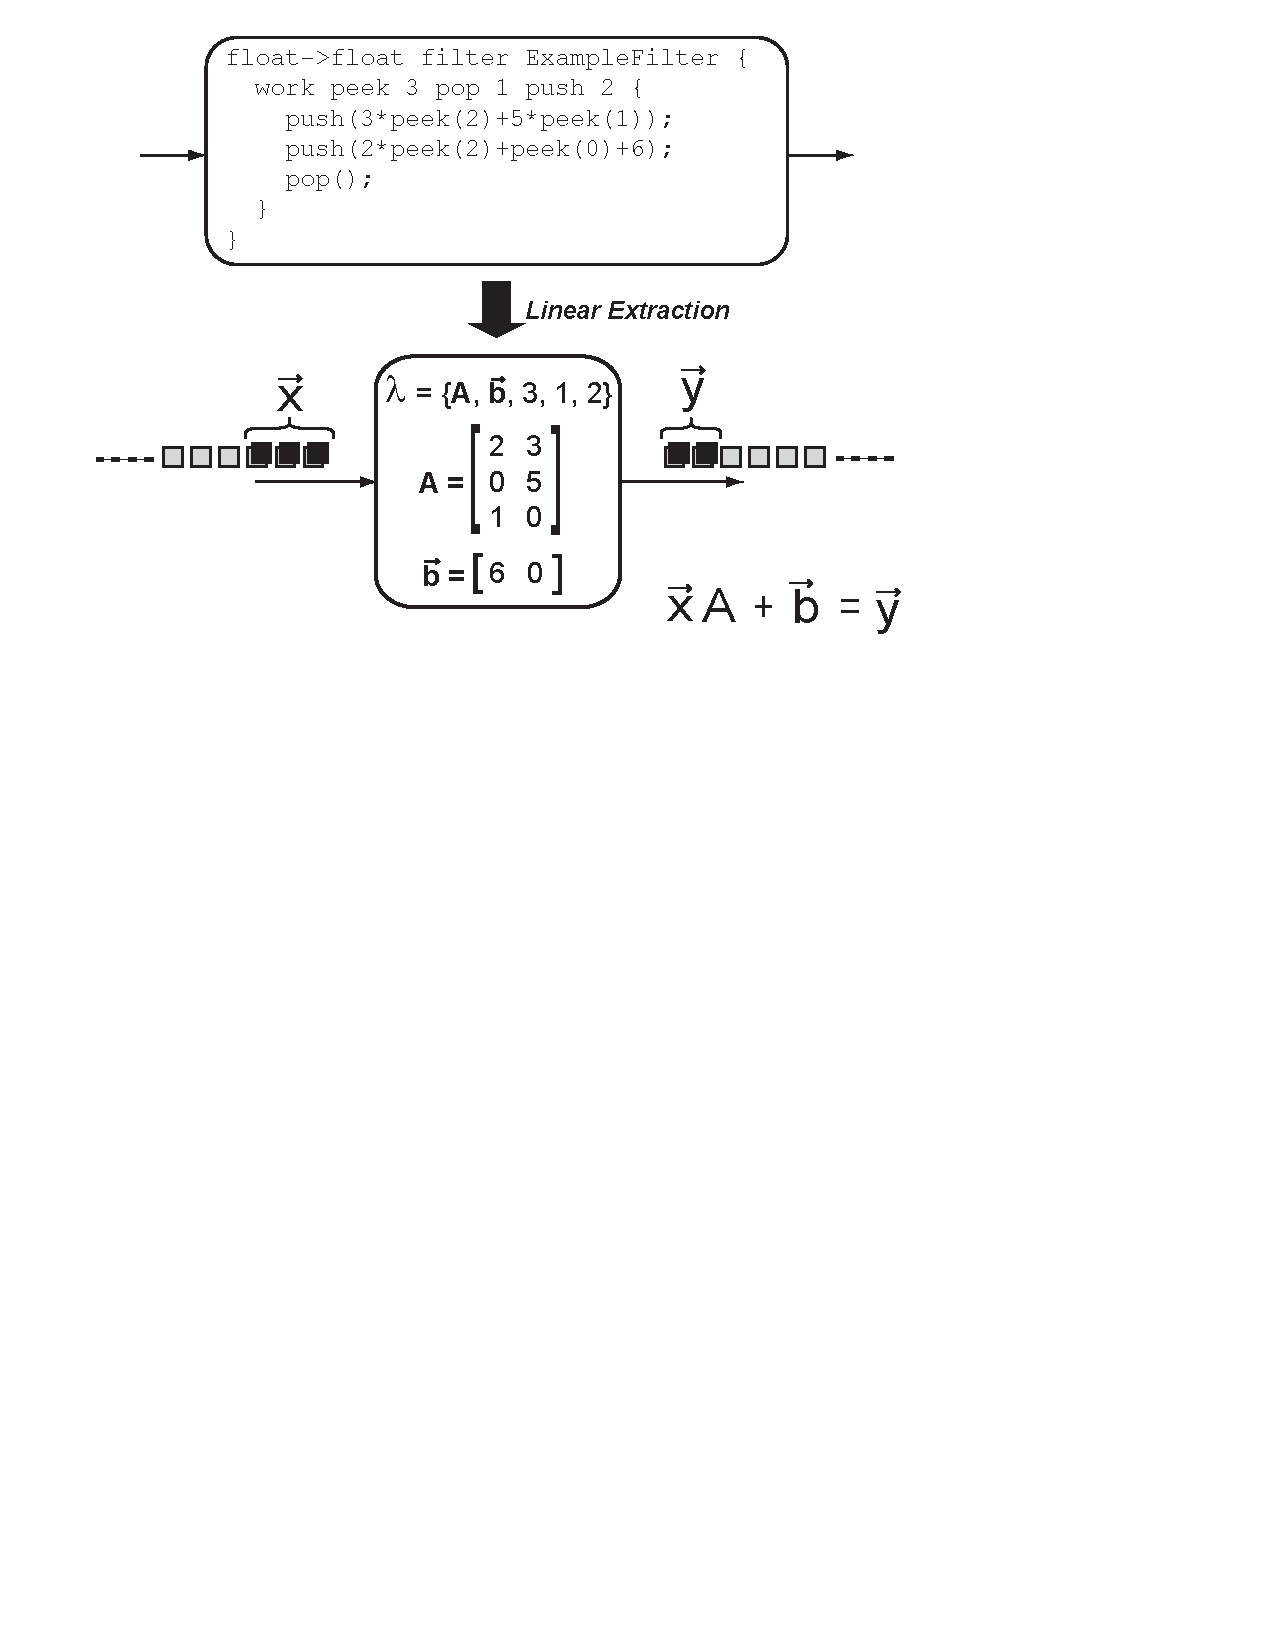
\includegraphics[width=3in]{thies3-2.pdf} % linear representation
    \vspace{-23pt}
    \caption{Representation of a linear node.~~~~~~\protect\label{fig:thies3-node}}
    \end{minipage}
    \hspace{0.1in}
    \begin{minipage}{2.4in}
    \includegraphics[width=2.4in]{thies3-5.pdf} % frequency translation
    \vspace{-18pt}
    \caption{Translation to frequency domain.\protect\label{fig:thies3-freq}}
    \end{minipage}
  \end{center}
  \vspace{-0.1in}
\end{figure}

\clearpage
Given the linear representations, we can exploit a common technique
from signal processing to translate linear nodes into the frequency
domain (see Figure~\ref{fig:thies3-freq}).  This optimization
transforms a linear node, which can be thought of as a convolution,
into a sequence of a Fast Fourier Transform (FFT), a vector-vector
multiply, and an Inverse FFT.  This technique offers an asymptotic
speedup from $O(n^2)$ for convolution in the time domain to $O(n
log(n))$ in the frequency domain.  As shown in
Figure~\ref{fig:thies3-combo}, adjacent linear nodes can also be
algebraically simplified into a single node by evaluating the product
of their matrices at compile time.  Note that if the matrix dimensions
do not match, one of the matrices must be expanded by simulating
multiple executions of the filter (see
Figure~\ref{fig:thies3-expand}).

\absection{Progress}

We have completed an implementation of linear extraction, frequency
translation, and algebraic simplification as part of the StreamIt
compiler.  In addition, the compiler includes a cost-benefit analysis
that determines when each of the optimizations should be applied.  The
analysis utilizes a dynamic programming algorithm to quickly consider
a large space of optimization scenarios and select the one likely to
yield the best performance.

Figure~\ref{fig:thies3-flops} illustrates the number of floating point
operations that are removed by linear combination, frequency
translation, and automatic selection using cost-benefit analysis.
This shows that, for our modest suite of programs, the transformations
eliminate many redundant operations in the code independent of the
target architecture.  Figure~\ref{fig:thies3-speedup} shows the
execution speedup on a Pentium III processor.  Using autoselect, the
average speedup is 450\%.

\absection{Future} An immediate extension of this work is to
``state-space analysis'' for linear filters that have internal state
that is updated in a linear fashion; this allows the analysis to
encompass feedback loops, as well as common filters such as the
Infinite Impulse Response (IIR).  We are also actively pursuing
domain-specific optimizations beyond the class of linear filters.  For
example, a numerical precision analysis could allow some ``lossy''
optimizations that cause slight alterations to the program's output
but remain within the allowed operating envelope.

\begin{figure}[t]
  \begin{center}
    \begin{minipage}{4.2in}
    \includegraphics[width=4.2in]{thies3-6.pdf} % linear combination
    \vspace{-20pt}
    \caption{Algebraic simplification of adjacent linear nodes.\protect\label{fig:thies3-combo}}
    \end{minipage}
    \begin{minipage}{1.9in}
      \vspace{-3pt}
    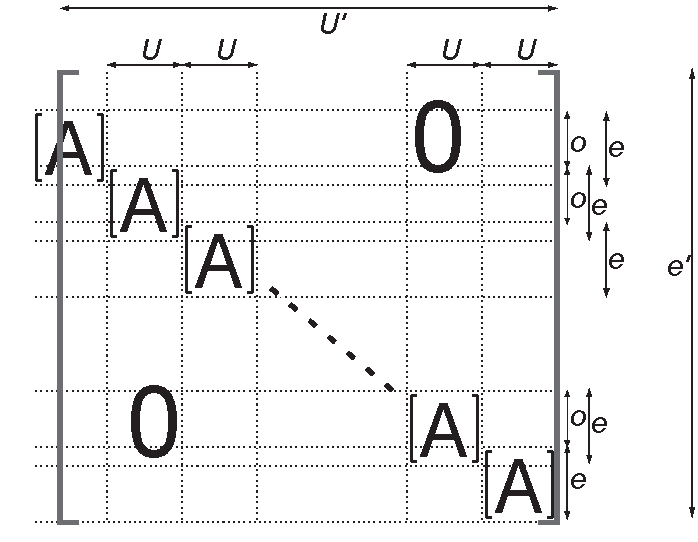
\includegraphics[width=1.9in]{thies3-1.pdf} % linear expansion
    \vspace{-20pt}
    \caption{Linear expansion.\protect\label{fig:thies3-expand}}
    \end{minipage}
    \\ ~ \vspace{12pt} \\
    \hfill
    \begin{minipage}{3in}
    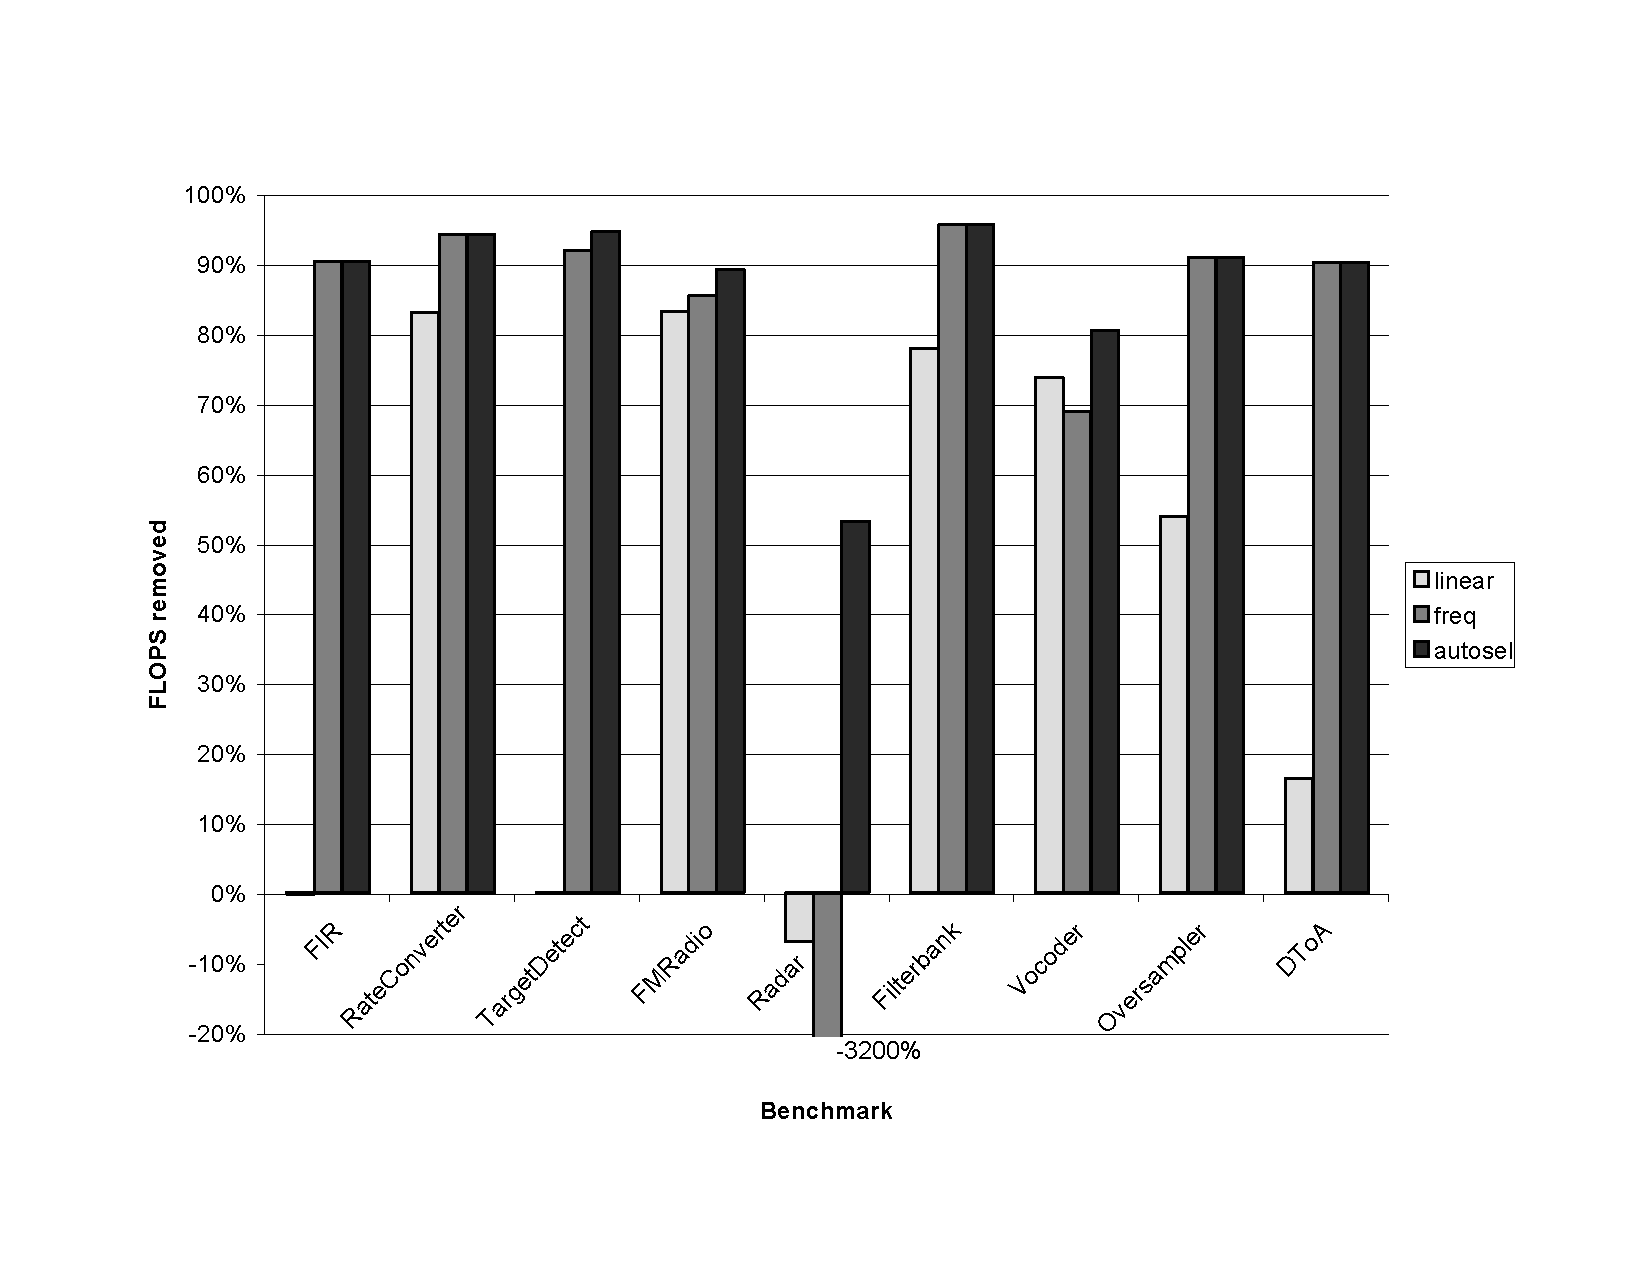
\includegraphics[width=3in]{thies3-4.pdf} % flops removal
    \vspace{-18.5pt}
    \caption{Elimination of floating point operations.\protect\label{fig:thies3-flops}}
    \end{minipage}
    \hfill
    \begin{minipage}{3in}
    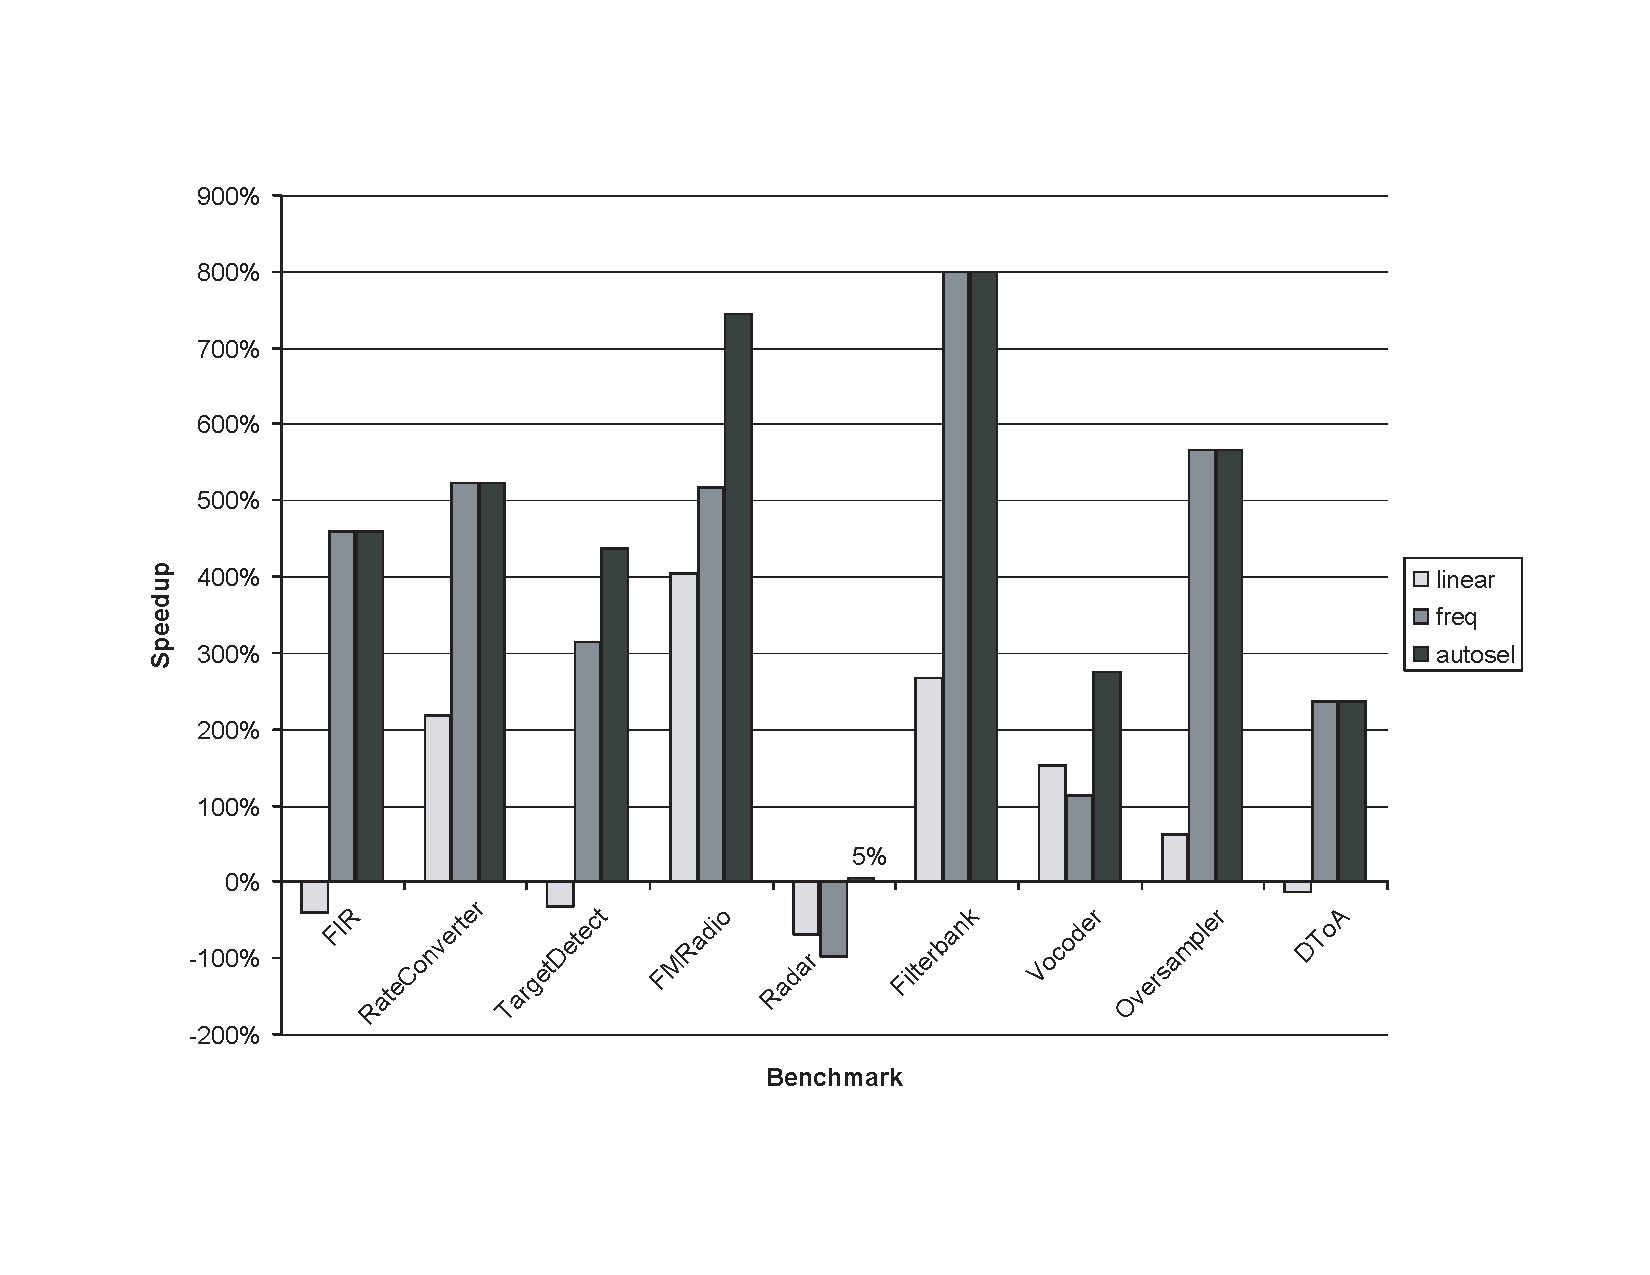
\includegraphics[width=3in]{thies3-3.pdf} % speedup
    \vspace{-16pt}
    \caption{Execution speedup.\protect\label{fig:thies3-speedup}}
    \end{minipage}
    \hfill
  \end{center}
  \vspace{-20pt}
\end{figure}

\absection{Research Support}
This work is supported in part by a grant from DARPA (PCA
F29601-04-2-0166), awards from NSF (CISE EIA-0071841, ITR ACI-0325297,
NGS CNS-0305453), and the MIT-Oxygen Project.

%% The abstract bibliographies should be done using bibtex.  Please
%% compile your bibtex entries into a single file with a distinguishing
%% name. The \absbibliography command is analogous to the \bibliography
%% command, taking a single argument, the name of your bibtex file, 
%% minus the .bib extention. The \bibliographystyle command should not
%% be used.  You can use a single bibliography file if you are submitting
%% multiple abstracts.  

\absbibliography{thies3}

\end{document}
